% Licensed under the Creative Commons Attribution Share Alike 4.0 International.
% See the LICENSE file in the repository root for full license text.

\section{学生应该已经掌握的基本能力}

在开始学习 CMake 之前,我假设读者掌握了最基础的 C++ 知识,具有编写单个 C++ 源文件的能力。为确保假设成立,我将首先演示程序设计课程中一套(可能)常见的操作流程:使用 Dev-C++ 集成开发环境编写一个简单的 C++ 程序并运行。读者不必亲自照此操作,但如果你对该流程并不熟悉,请考虑复习你的程序设计课程。

\begin{enumerate}
	\item 下载并安装 Dev-C++。目前,Dev-C++ 的代码仓库已迁移至 GitHub\footnote{网址:\url{https://github.com/Embarcadero/Dev-Cpp}。},最新的版本为 6.3,可以从发布页面\footnote{网址:\url{https://github.com/Embarcadero/Dev-Cpp/releases/tag/v6.3}。}得到安装包的下载地址:\url{https://github.com/Embarcadero/Dev-Cpp/releases/download/v6.3/Embarcadero_Dev-Cpp_6.3_TDM-GCC_9.2_Setup.exe}。下载该安装包,并以默认配置安装。

	\item 新建源文件并编写代码。安装完成后,打开 Dev-C++,可以看到图 \ref{fig:dev-cpp-1} 所示的界面。点击“新文件”,编写图 \ref{fig:dev-cpp-2} 所示的代码,然后保存。

	\begin{figure}
		\centering
		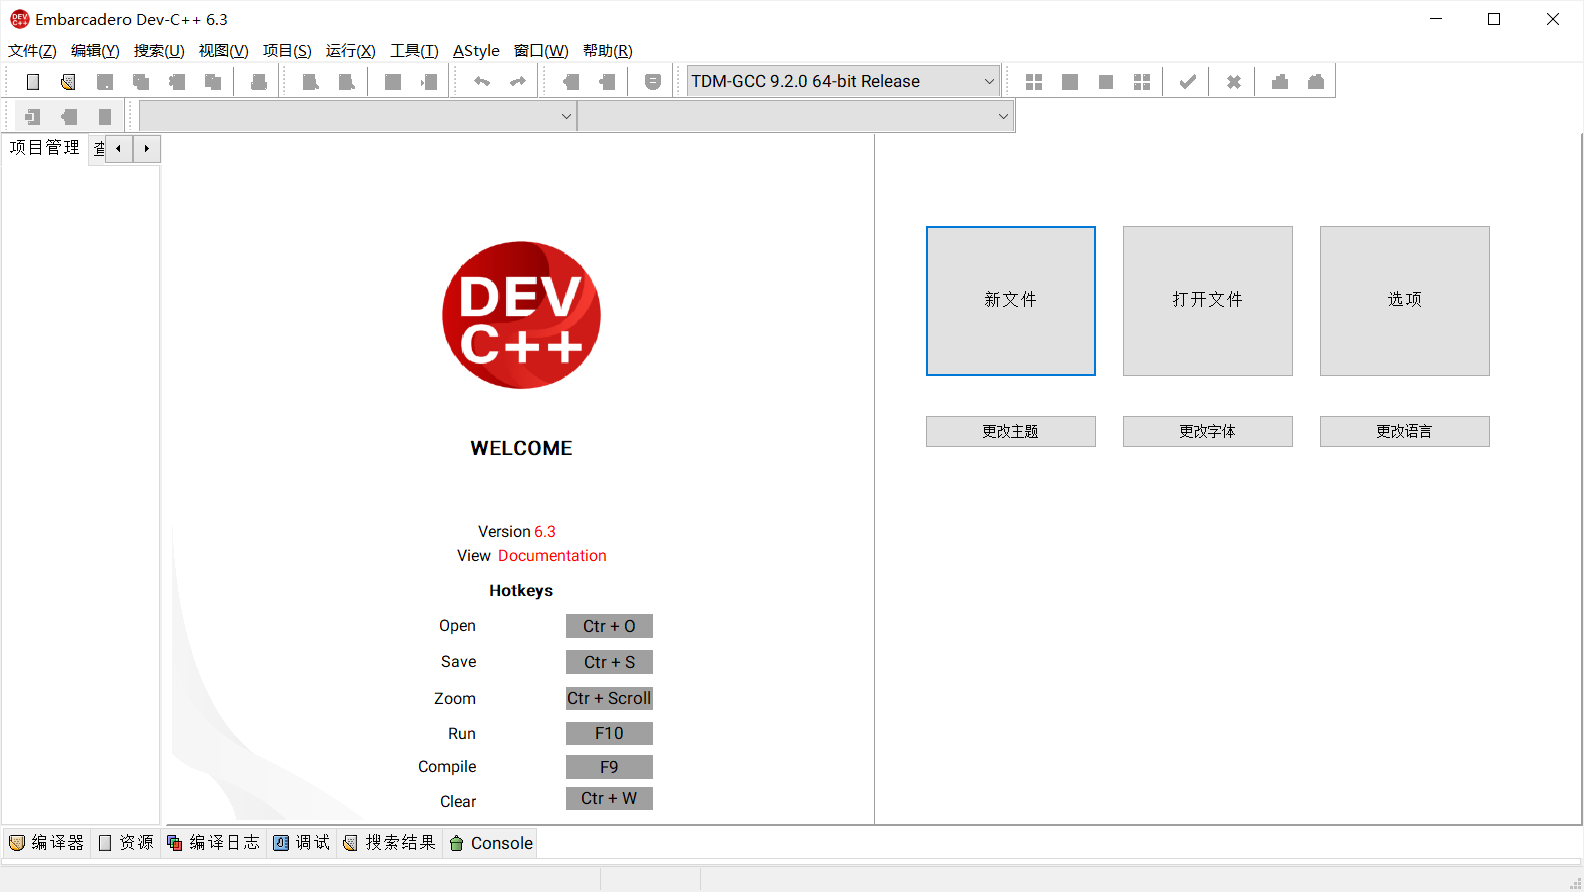
\includegraphics[width=\linewidth]{assets/dev-cpp-1}
		\caption{Dev-C++ 启动界面。}
		\label{fig:dev-cpp-1}
	\end{figure}

	\begin{figure}
		\centering
		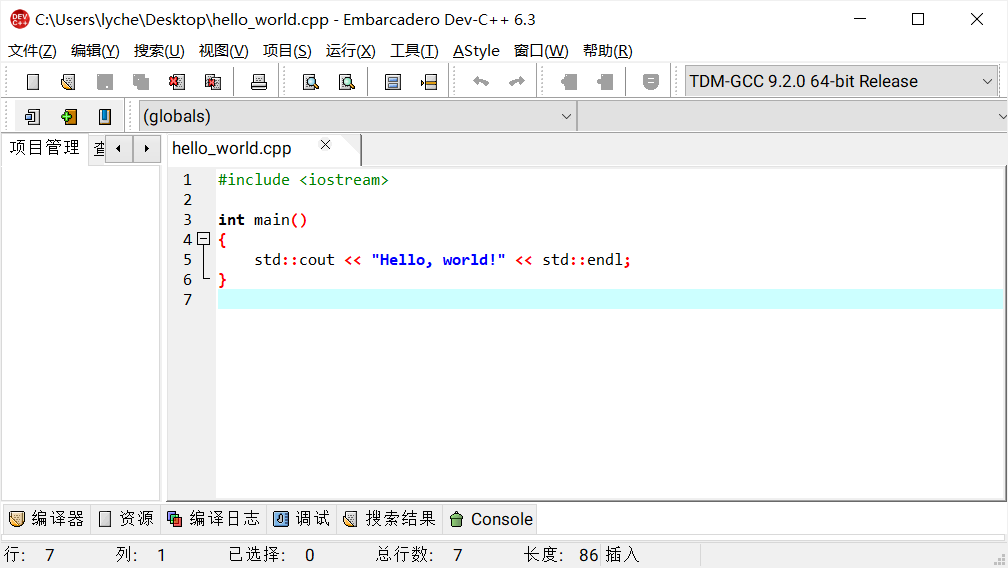
\includegraphics[width=\linewidth]{assets/dev-cpp-2}
		\caption{在 Dev-C++ 中编写一个简单的 C++ 源文件。}
		\label{fig:dev-cpp-2}
	\end{figure}

	\item 编译并运行代码。点击菜单栏中的“运行”、“编译运行”,可以看到“编译日志”窗口弹出,如图 \ref{fig:dev-cpp-3} 所示。编译结束后,程序自动运行,运行结果如图 \ref{fig:dev-cpp-4} 所示。

	\begin{figure}
		\centering
		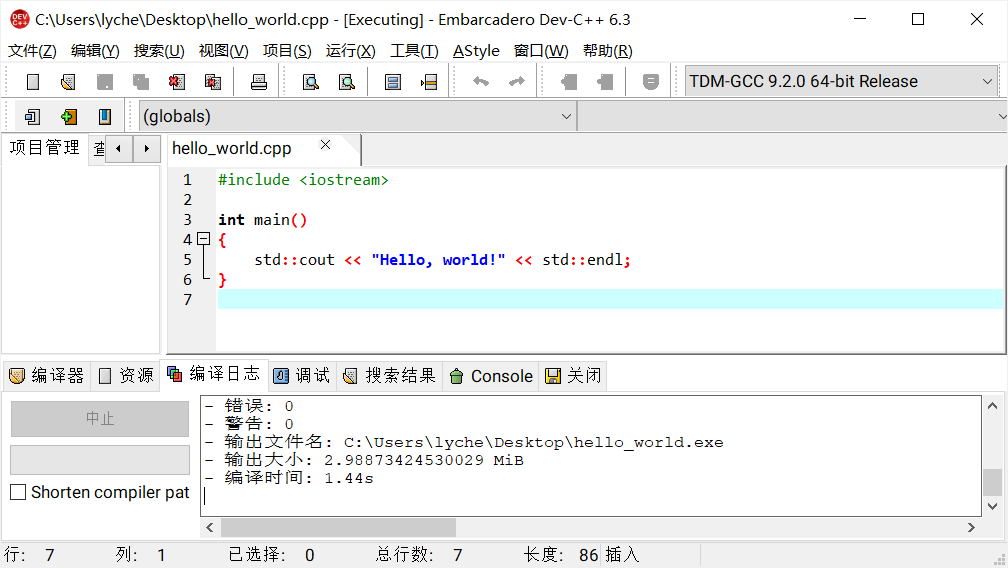
\includegraphics[width=\linewidth]{assets/dev-cpp-3}
		\caption{编译程序后,Dev-C++ 弹出“编译日志”窗口。}
		\label{fig:dev-cpp-3}
	\end{figure}

	\begin{figure}
		\centering
		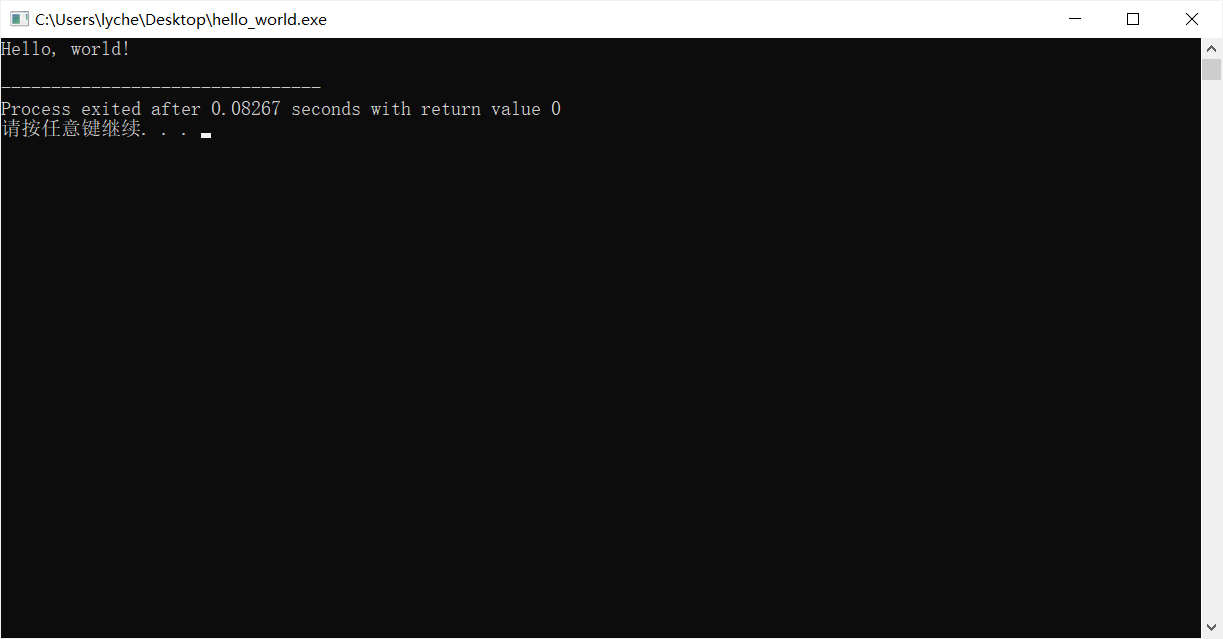
\includegraphics[width=\linewidth]{assets/dev-cpp-4}
		\caption{控制台程序的运行结果。}
		\label{fig:dev-cpp-4}
	\end{figure}
\end{enumerate}

值得关注的是 Dev-C++ 的编译日志。

\begin{lstlisting}[language={}]
编译单个文件...
--------
- 文件名: C:\Users\lyche\Desktop\hello_world.cpp
- 编译器名: TDM-GCC 9.2.0 64-bit Release

处理 C++ 源文件...
--------
- C++ 编译器: C:\Program Files (x86)\Embarcadero\Dev-Cpp\TDM-GCC-64\bin\g++.exe
- 命令: g++.exe "C:\Users\lyche\Desktop\hello_world.cpp" -o "C:\Users\lyche\Desktop\hello_world.exe"  -I"C:\Program Files (x86)\Embarcadero\Dev-Cpp\TDM-GCC-64\include" -L"C:\Program Files (x86)\Embarcadero\Dev-Cpp\TDM-GCC-64\lib" -static-libgcc

编译结果...
--------
- 错误: 0
- 警告: 0
- 输出文件名: C:\Users\lyche\Desktop\hello_world.exe
- 输出大小: 2.98873424530029 MiB
- 编译时间: 1.44s
\end{lstlisting}

从以上编译日志可以看到,Dev-C++ IDE 的职责是帮助我们调用编译器,并且以命令行的形式向编译器传入大量参数。上例包含的参数有:

\begin{itemize}
	\item 参与编译的源文件的路径。
	\item \lstinline[language={}]{-o}:输出文件的路径。
	\item \lstinline[language={}]{-I}:额外的包含目录。
	\item \lstinline[language={}]{-L}:额外的链接目录。
	\item \lstinline[language={}]{-static-libgcc}:指定链接 libgcc 库的方式为静态链接。
\end{itemize}

几乎所有实际的工程都存在不止一个源文件。可以预见,编译这些工程所需的参数会比上例复杂许多。在本章的剩余部分,我们将上手感受它们的复杂性。
